\section{Description of Preliminary Experiments}
\label{Se:perf}


\smartpar{Methodology and Experimental Setup}
%
We conducted our experiments on server with two Intel(R) Xeon(R) CPU E5-2690 0 @ 2.90GHz (16 cores) CPUs with 132GB of RAM. The server runs version
6.6 of the CentOS Linux distribution, and has the Sun 64-Bit 1.8 Java virtual machine (JVM) installed.

In our experiments, we varied two aspects of parallel execution: \emph{workload size}, measured as the number of transactions executed by a given thread for a fixed number $n$ of threads, and \emph{concurrency level}, setting the number of threads for a fixed workload size. For the former, we fixed $n=8$ and varied the number of transactions, where each transaction executes a single client method. For the latter, we experimented with 2 to 32 threads with workload size fixed at 10.
%\begin{itemize}
	%\item
%	\emph{Workload size:} For a fixed number $n$ of threads, where $n=8$,  the workload size is varied. The workload is measured as the number of transactions executed by a given thread, where a single transaction consists of the invocation of a particular method. All inputs share the same key(s).
%	\item \underline{Concurrency level:} For a fixed workload size, set at 10%\pengtodo{please confirm}
%	, the number of threads is varied along the range of 2 to 32 threads.  
%\end{itemize}
For statistical soundness, we report the average performance results across 10 independent repetitions of each experiment.

We compare our technique against two competing solutions: (i) a pessimistic concrete-level variant of STM, as available via version 1.3 of the Deuce STM (the latest version)\footnote{
		\url{https://github.com/DeuceSTM/DeuceSTM}
	}, and (ii)  a lock-based synchronization algorithm boosted with {\sf Map} semantics \cite{ppopp/HerlihyK08}, such that the locks are of the same grain as their corresponding abstract locks in boosted STM.

\smartpar{Subjects}
%
Our benchmark suite consists of four subjects, all of which are taken from popular open-source code bases and have been used in past studies on concurrency \cite{oopsla/ShachamBASVY11,issta/ShachamYGABSV14}.
%\begin{itemize}
	%\item 
	Apache Tomcat is web-app container in wide deployment. Within it, we consider {\sf ApplicationContext}, which is a concrete representation of a web application's execution environment.
	dyuproject is a framework for development of Java web applications. We experiment with {\sf StandardConvertorCache}, which handles conversion of objects to/from JSON format.
	Flexive is a next-generation content repository for development of web apps, in particular in an enterprise setting. We have included {\sf FxValueRendererFactory} from it, which is responsible to render transparently certain objects in a language.
	Finally, Gridkit is a library containing utilities related to in-memory data grids. In it, {\sf ReflectionPofSerializer} is a concurrent data structure that supports generic POF serialization via reflection.
%\end{itemize}

We have extracted two concurrent methods out of each benchmark. These were selected based on past studies that report on concurrency bugs in, and interference between, the selected methods \cite{oopsla/ShachamBASVY11}. 
%
As an illustration, in Figure \ref{Fi:gridkitPair} we present the method pair from Gridkit. In both of these methods, the intended atomic ``put-if-absent'' behavior (available as the {\sf putIfAbsent} API) is misimplemented due to the separation between the {\sf get} and {\sf put} calls. (We omit other method pairs for lack of space.)

\begin{figure}[tb]
%	\begin{lstlisting}
%protected Object internalDeserialize(PofReader in) 
%   throws IOException {
% Class type = in.getPofContext().getClass(in.getUserTypeId());
% ObjectFormat format = formats.get(type);
% if (format == null) {
%  try {
%   format = new ObjectFormat(type);
%  } catch (Exception e) {
%   throw new IOException(... + type.getName(), e); }
%  formats.put(type, format); }
%  Object result = resolve(format.deserialize(in));
%  return result; }
%	\end{lstlisting}
%
%	\begin{lstlisting}
%protected void internalSerialize(PofWriter out,Object origVal) 
%   throws IOException {
% Object value = replace(origVal);
% Class type = value.getClass();
% ObjectFormat format = formats.get(type);
% if (format == null) {
%  try {
%   format = new ObjectFormat(type);
%  } catch (Exception e) {
%   throw new IOException(... + type.getName(), e); }
%  formats.put(type, format); }
% format.serialize(out, value); }
%	\end{lstlisting}
\begin{lstlisting}
Object internalDeserialize(PofReader in) {
  Class t = in.getPofContext().getClass(in.getUserTypeId());
  ObjectFormat f = formats.get(t);
  if (f == null) { f = new ObjectFormat(t); formats.put(t, f); }
  return resolve(f.deserialize(in)); }

void internalSerialize(PofWriter out, Object o) {
  Object v = replace(o); Class t = v.getClass();
  ObjectFormat f = formats.get(t);
  if (f == null) { format = new ObjectFormat(t); formats.put(t, f); }
  format.serialize(out, v); }
\end{lstlisting}
	\caption{\label{Fi:gridkitPair}Concurrent methods from the Gridkit benchmark}
\end{figure}



%The left-hand-side charts correspond to the first measurement, where we increase the size of the workload while fixing the number of threads. The right-hand-side graphs correspond to a fixed-size workload executed by each of the transactions, where the number of threads is variable.

%
We depict the detailed performance results in Figure\ref{fig:perf}, where for each benchmark we plot the results when increasing the size of the workload while fixing the number of threads (on the left), and when varying the number of threads (on the right).
Each plot presents a two column diagram, corresponding to STM and corrective synchronization (left/black and right/gray, respectively), which indicates the relative gain thanks to these approaches in comparison with lock-based synchronization. Indeed, the lock-based solution is overly conservative, yielding roughly a linear trend line of decrease in performance as either workload size or the number of threads increases.

\newcommand\mywidth{0.5 \textwidth}
\begin{figure*}
  \rotatebox{90}{\scriptsize Tomcat {\sf ApplicationContext}}
  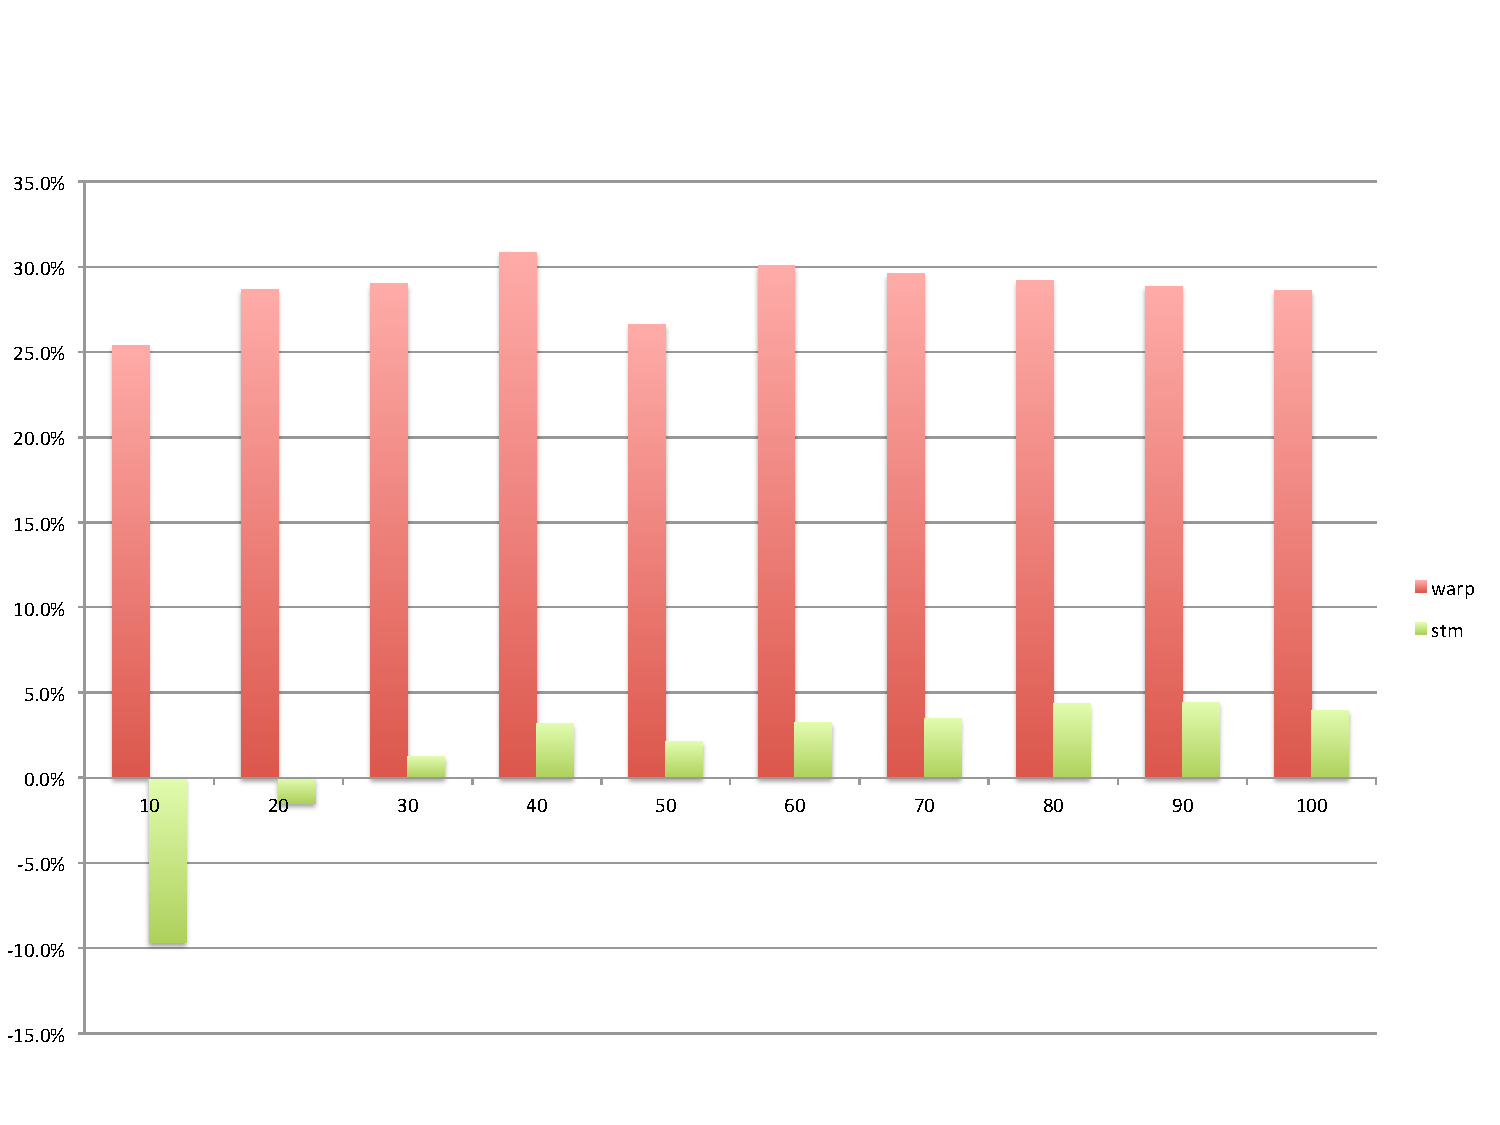
\includegraphics[width=\mywidth]{../../eval/32threads/case1it.pdf}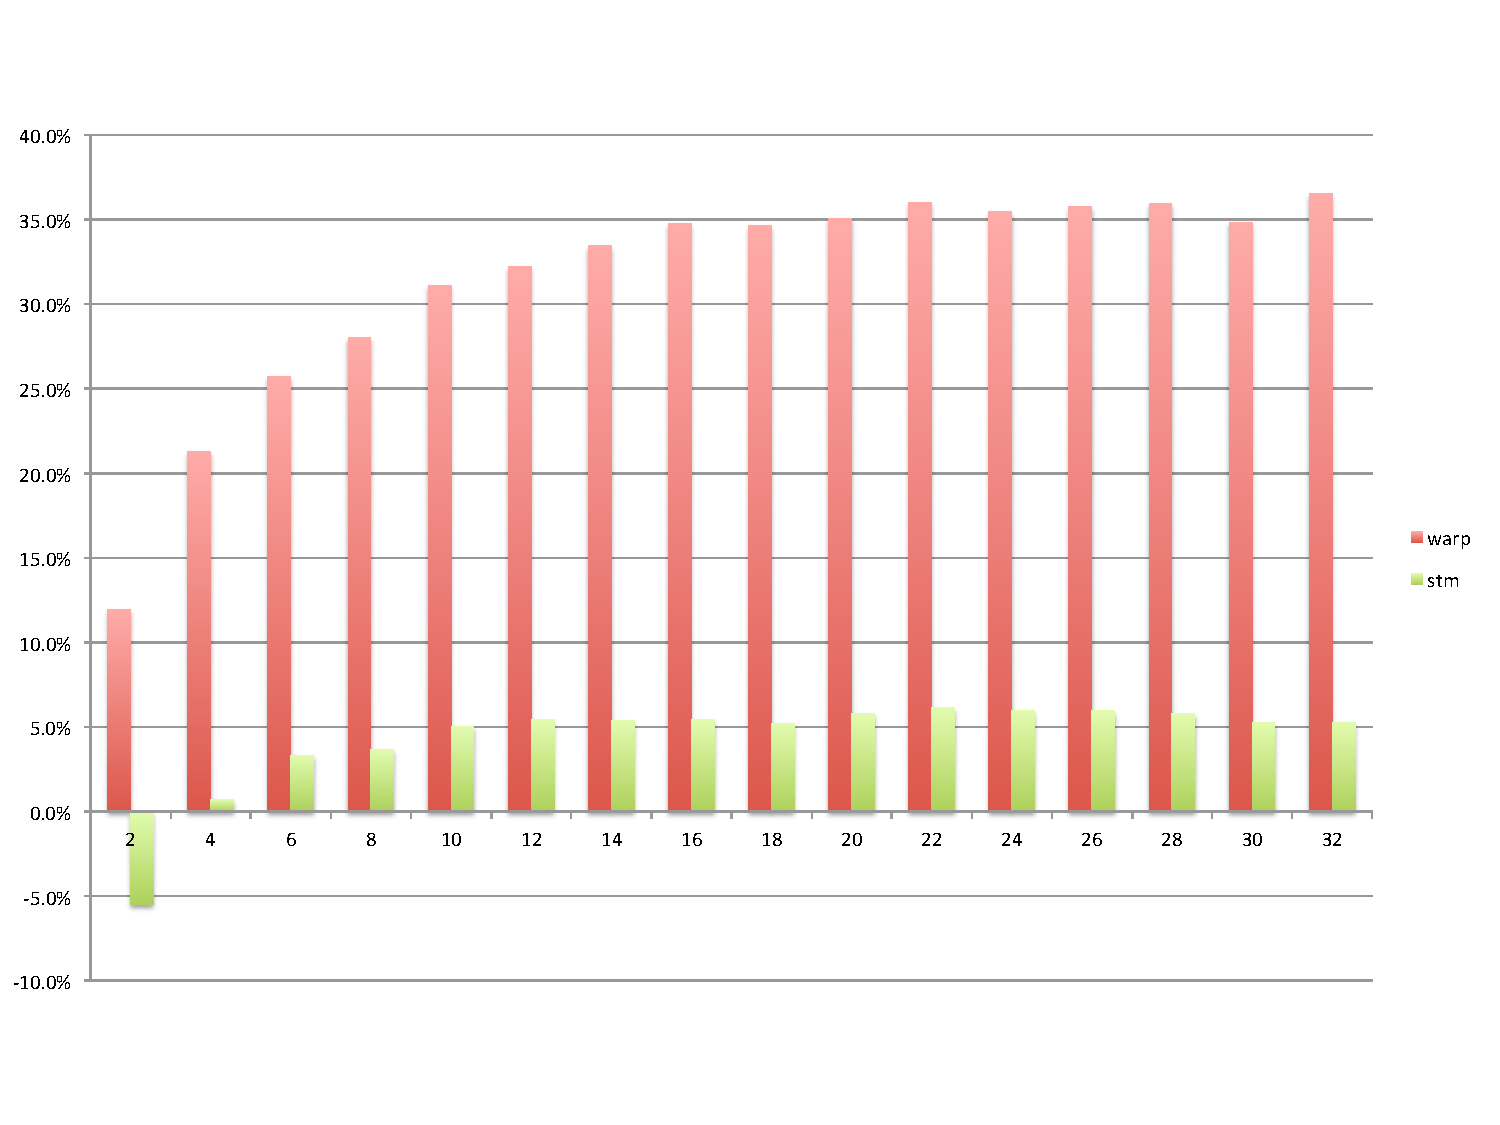
\includegraphics[width=\mywidth]{../../eval/32threads/case1th.pdf}

  \medskip
  \rotatebox{90}{\scriptsize dyuproject {\sf StdConvertorCache}}
  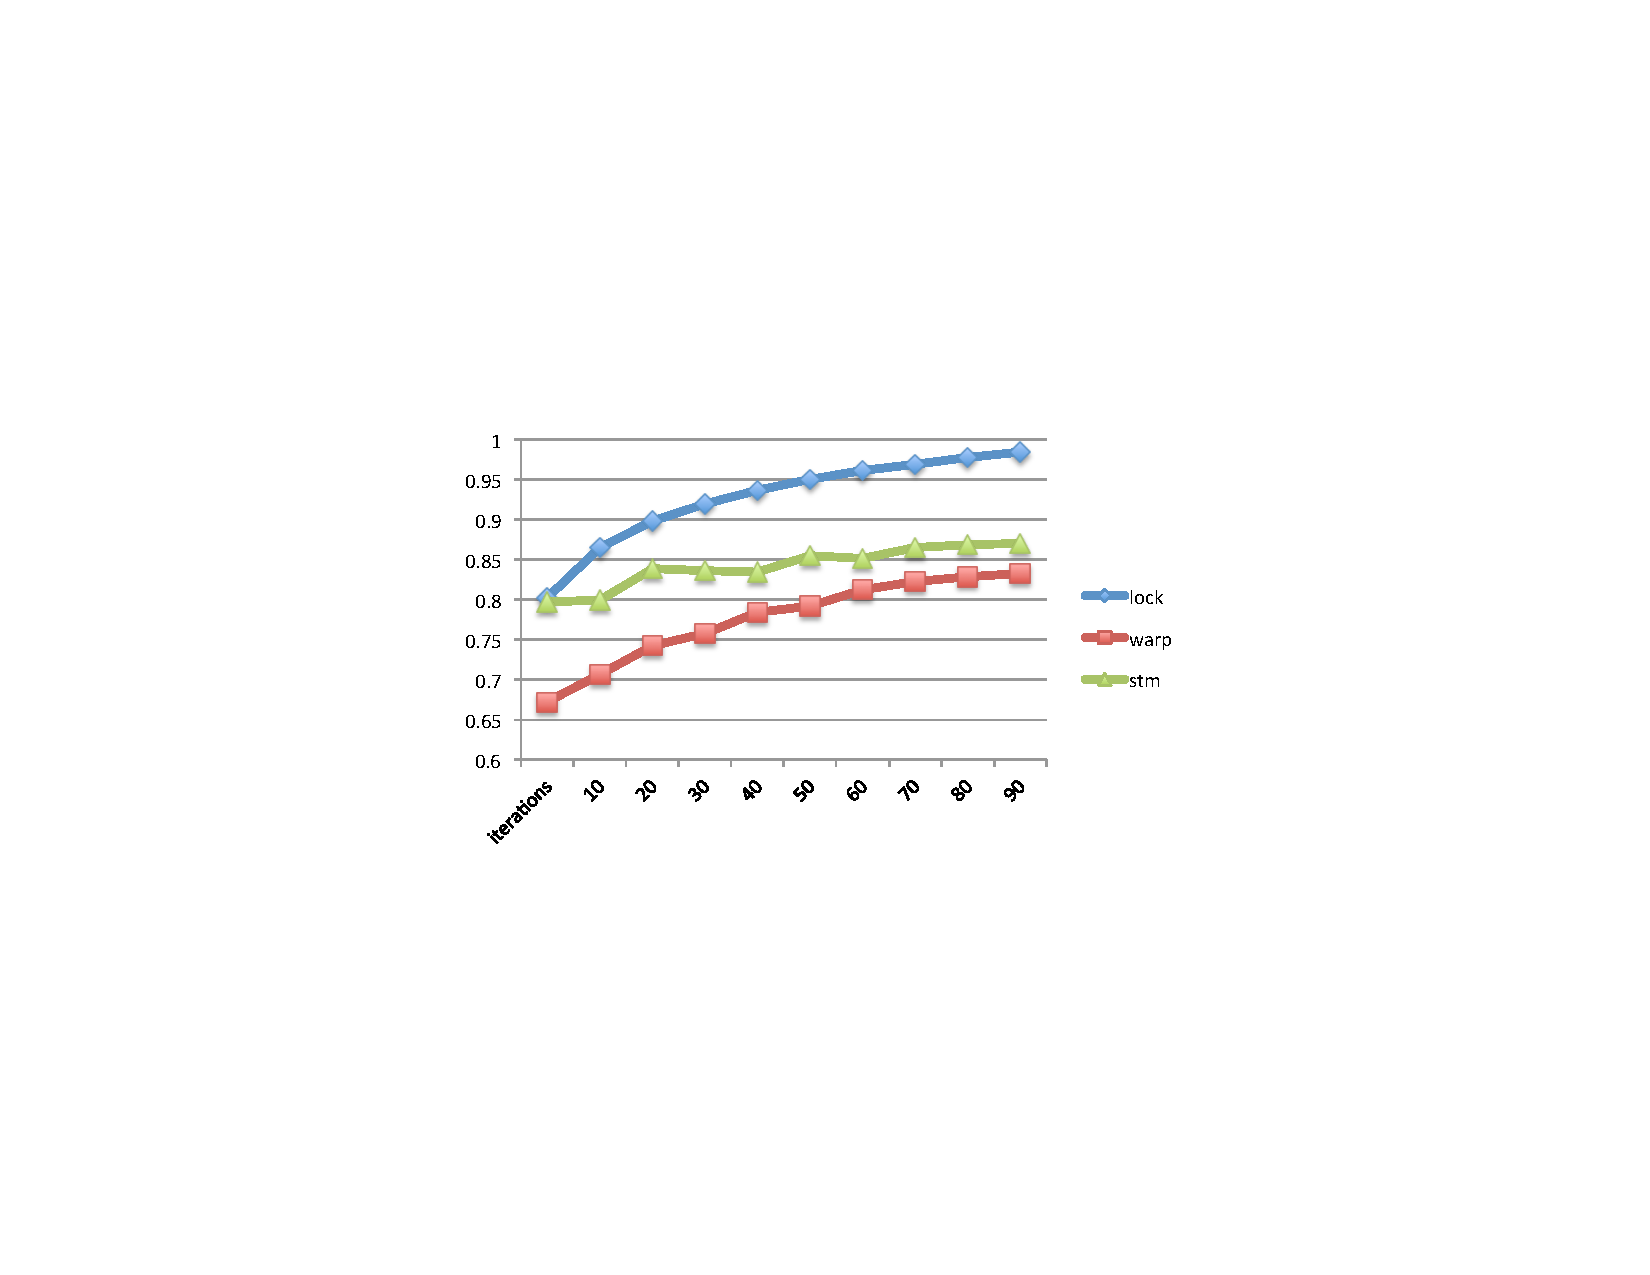
\includegraphics[width=\mywidth]{../../eval/32threads/case2it.pdf}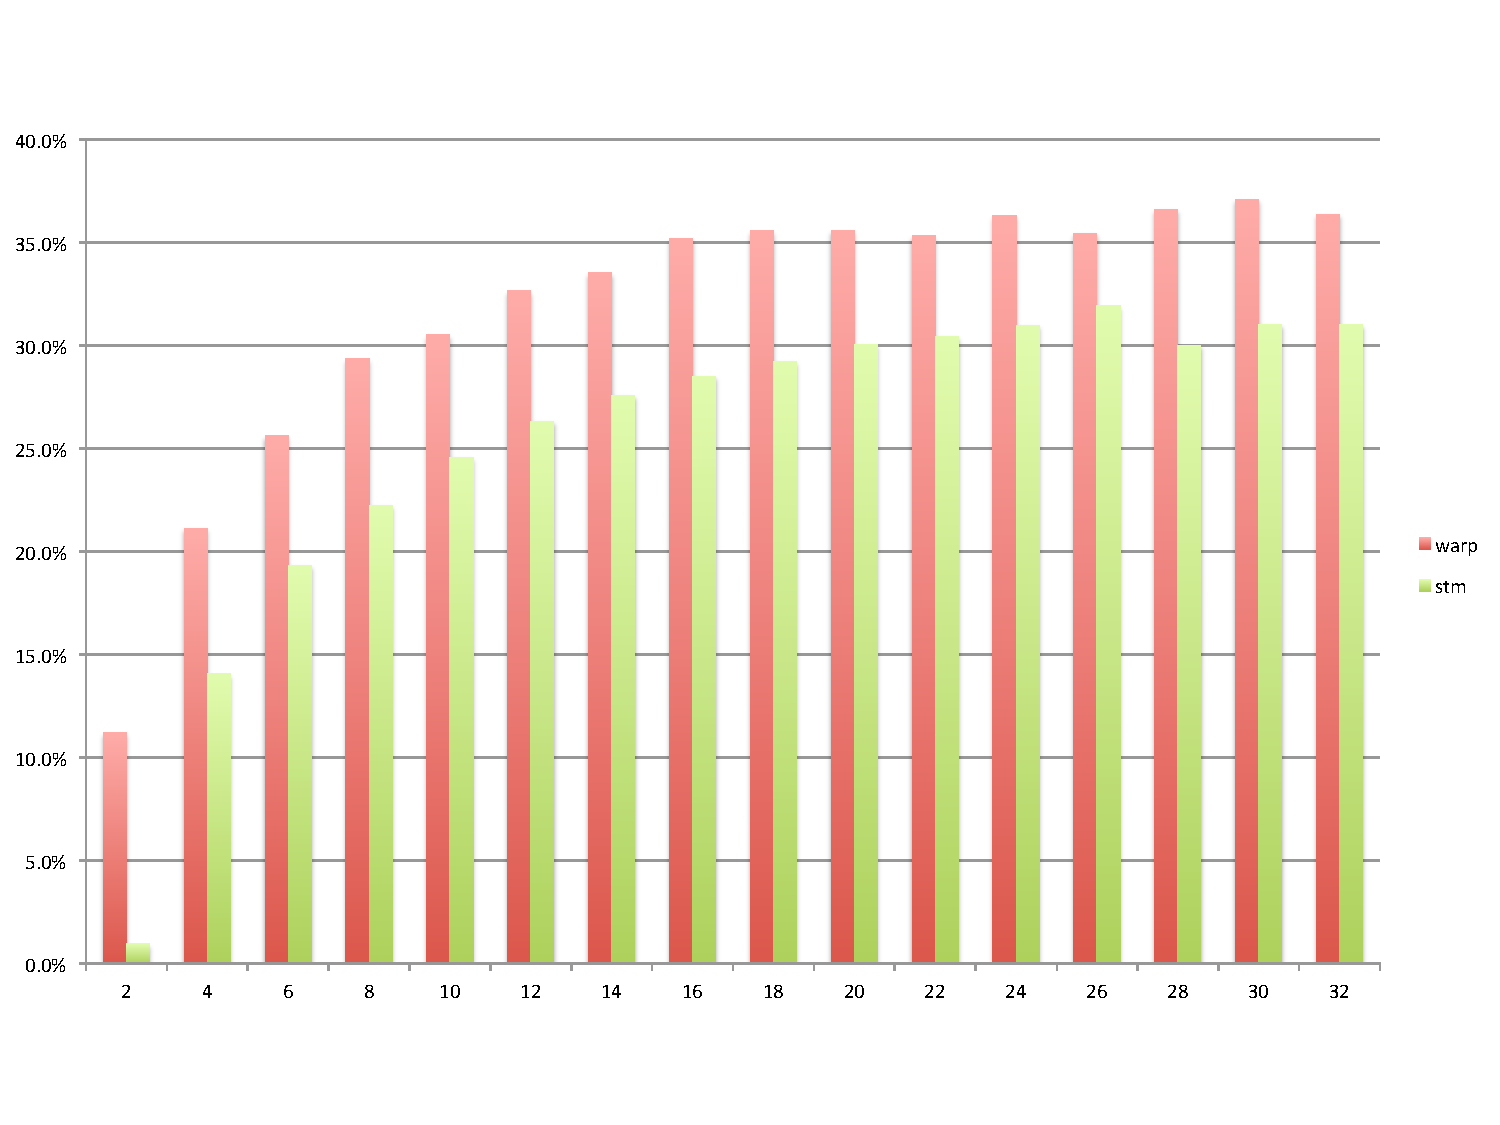
\includegraphics[width=\mywidth]{../../eval/32threads/case2th.pdf}

  \medskip
  \rotatebox{90}{\scriptsize Flexive {\sf FxValueRendererFactory}}
  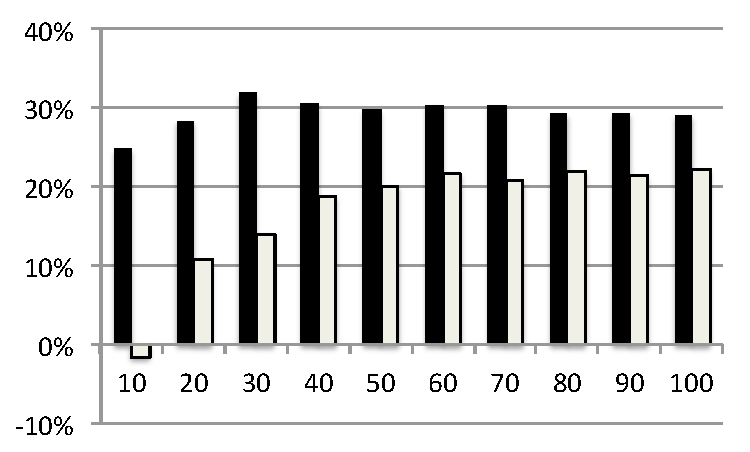
\includegraphics[width=\mywidth]{../../eval/32threads/case3it.pdf}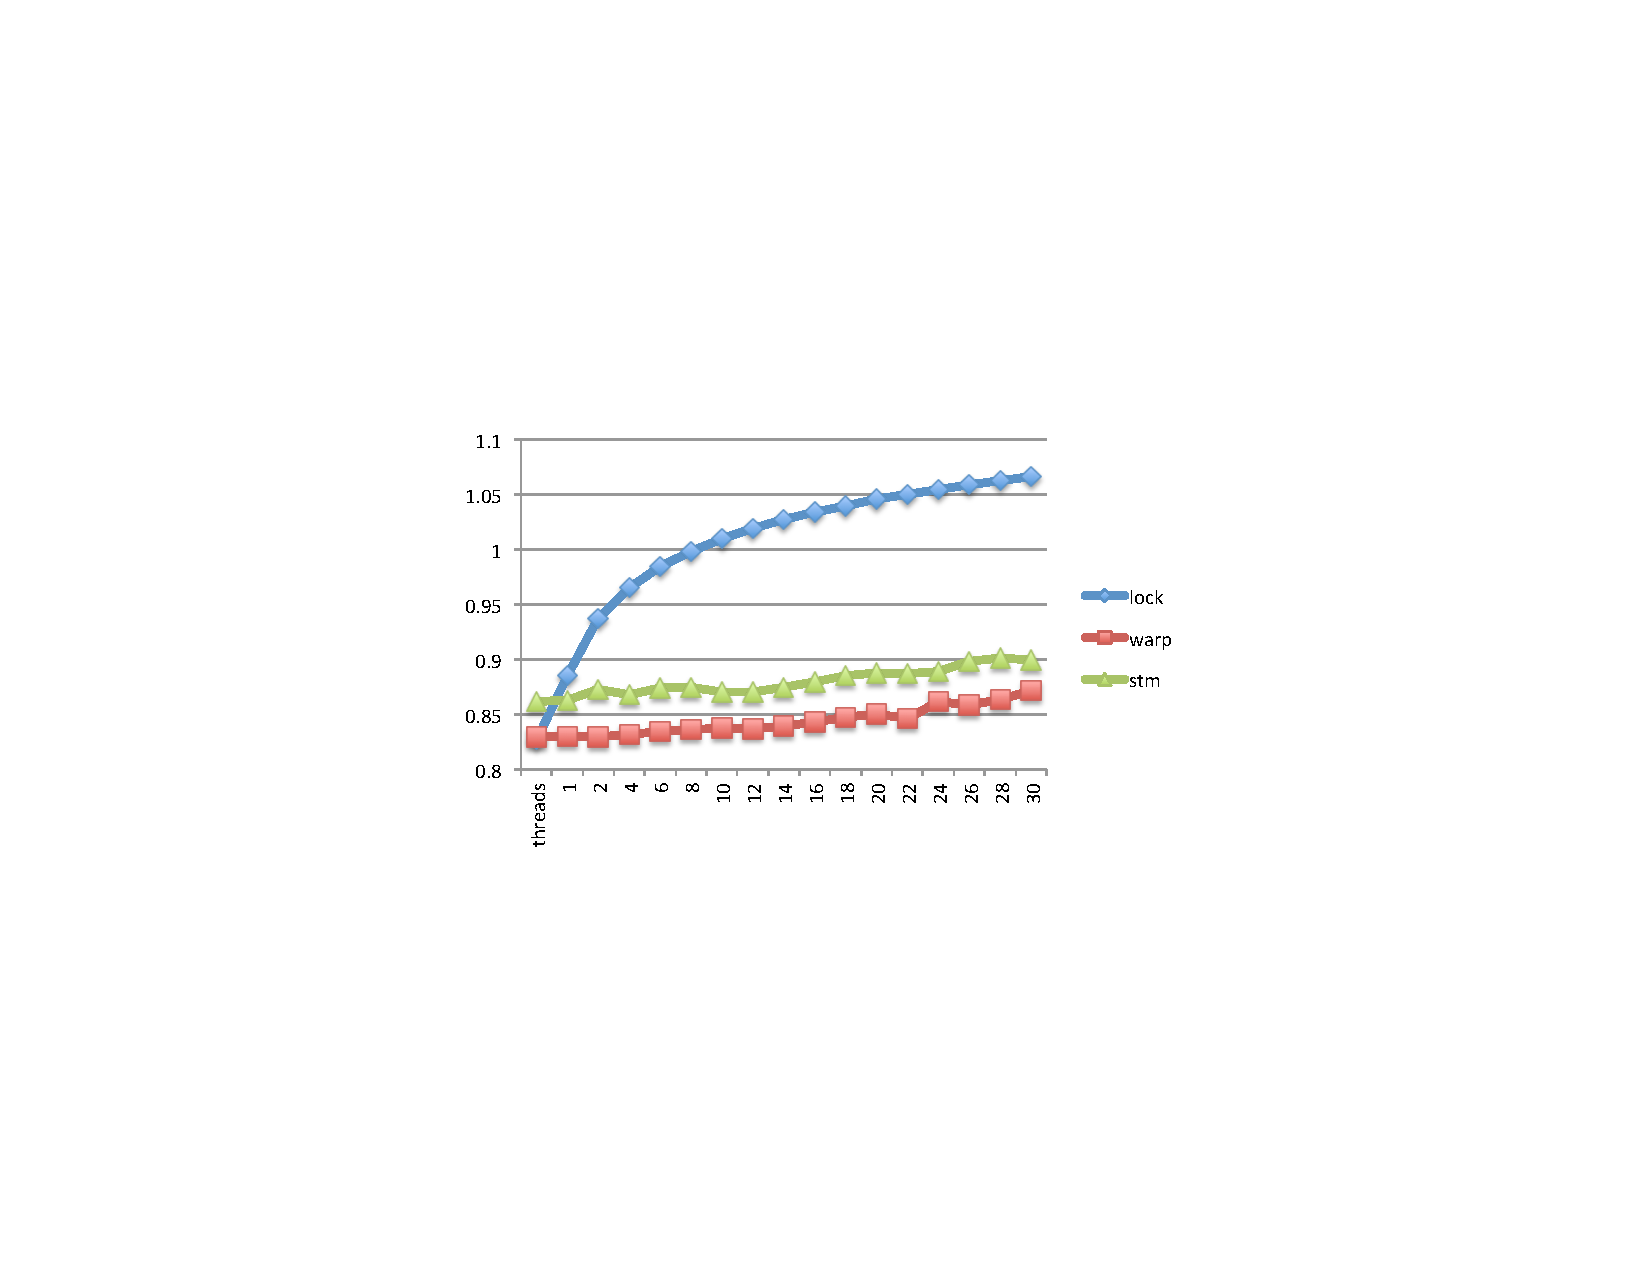
\includegraphics[width=\mywidth]{../../eval/32threads/case3th.pdf}
%\end{figure*}
%\vspace{-1cm}
%\begin{figure*}

  \medskip
  \rotatebox{90}{\scriptsize Gridkit {\sf ReflectionPofSerializer}}
  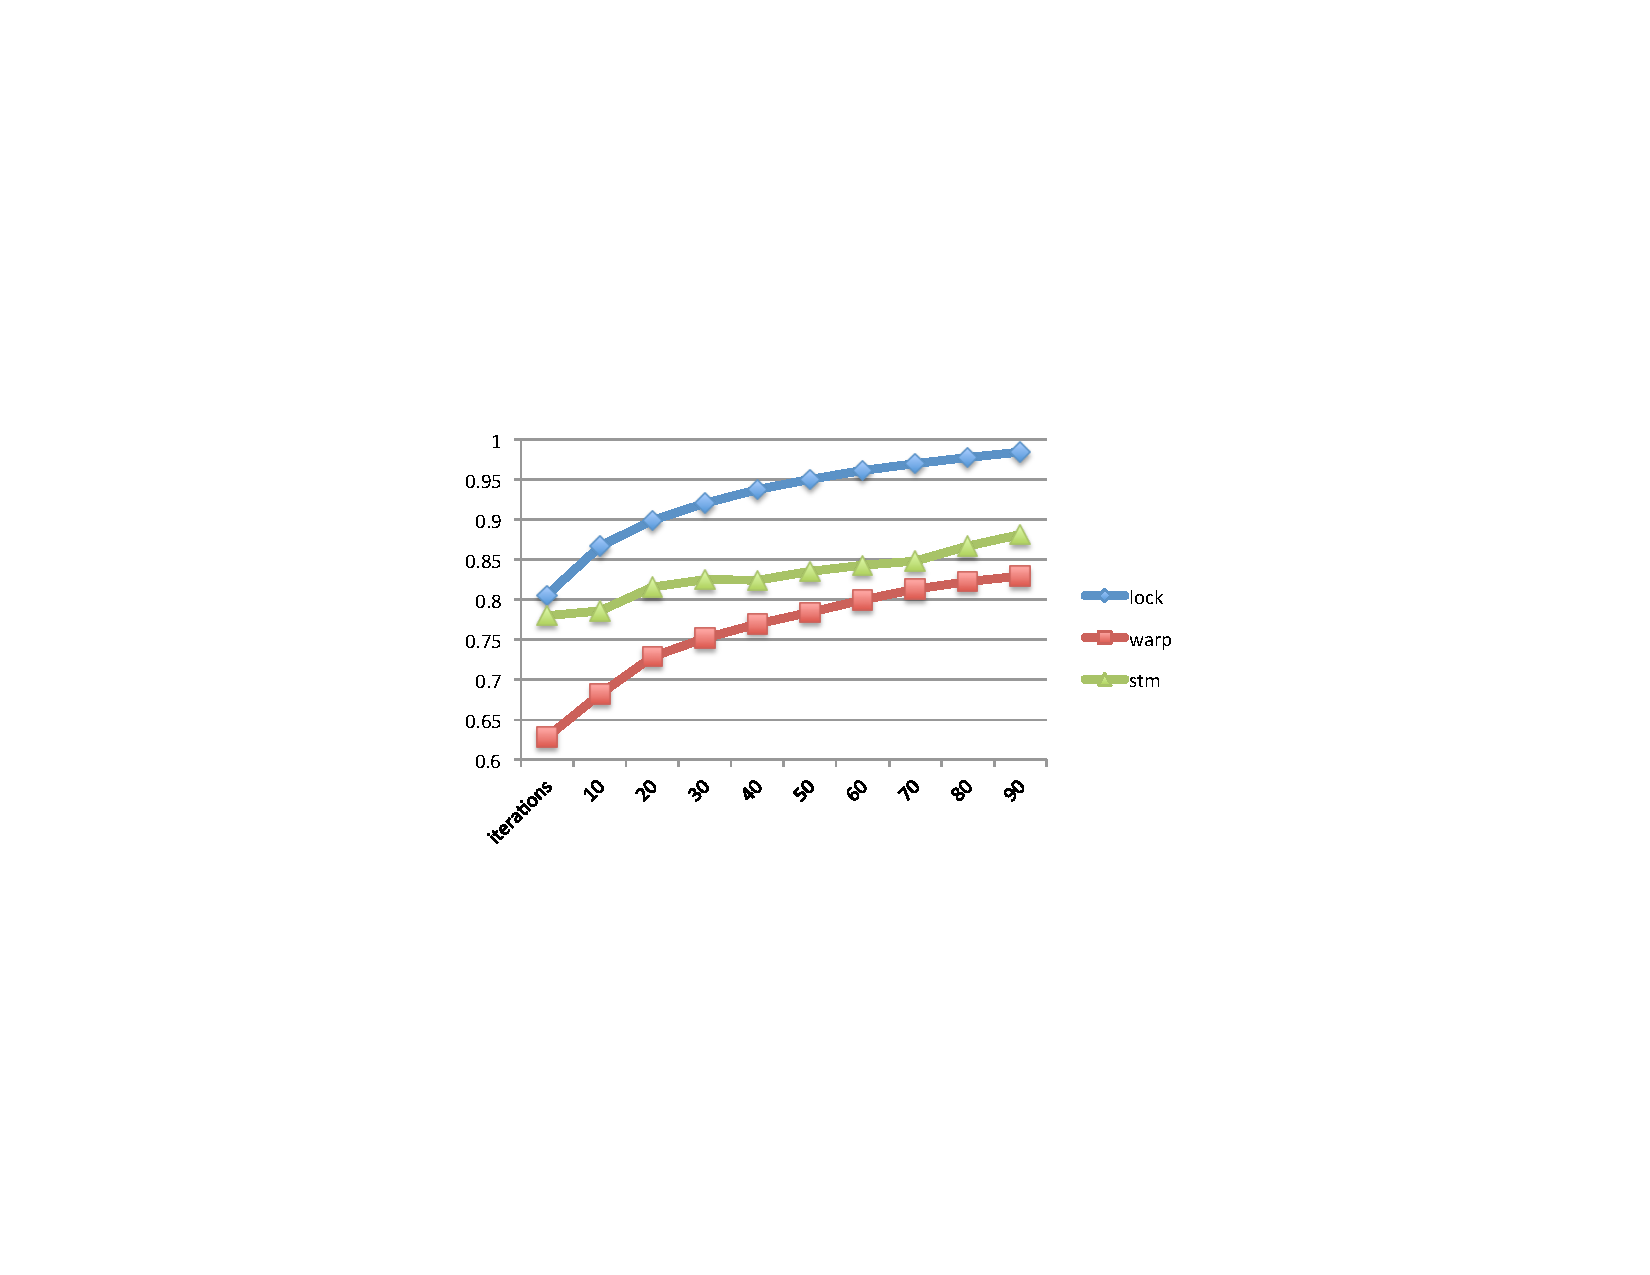
\includegraphics[width=\mywidth]{../../eval/32threads/case4it.pdf}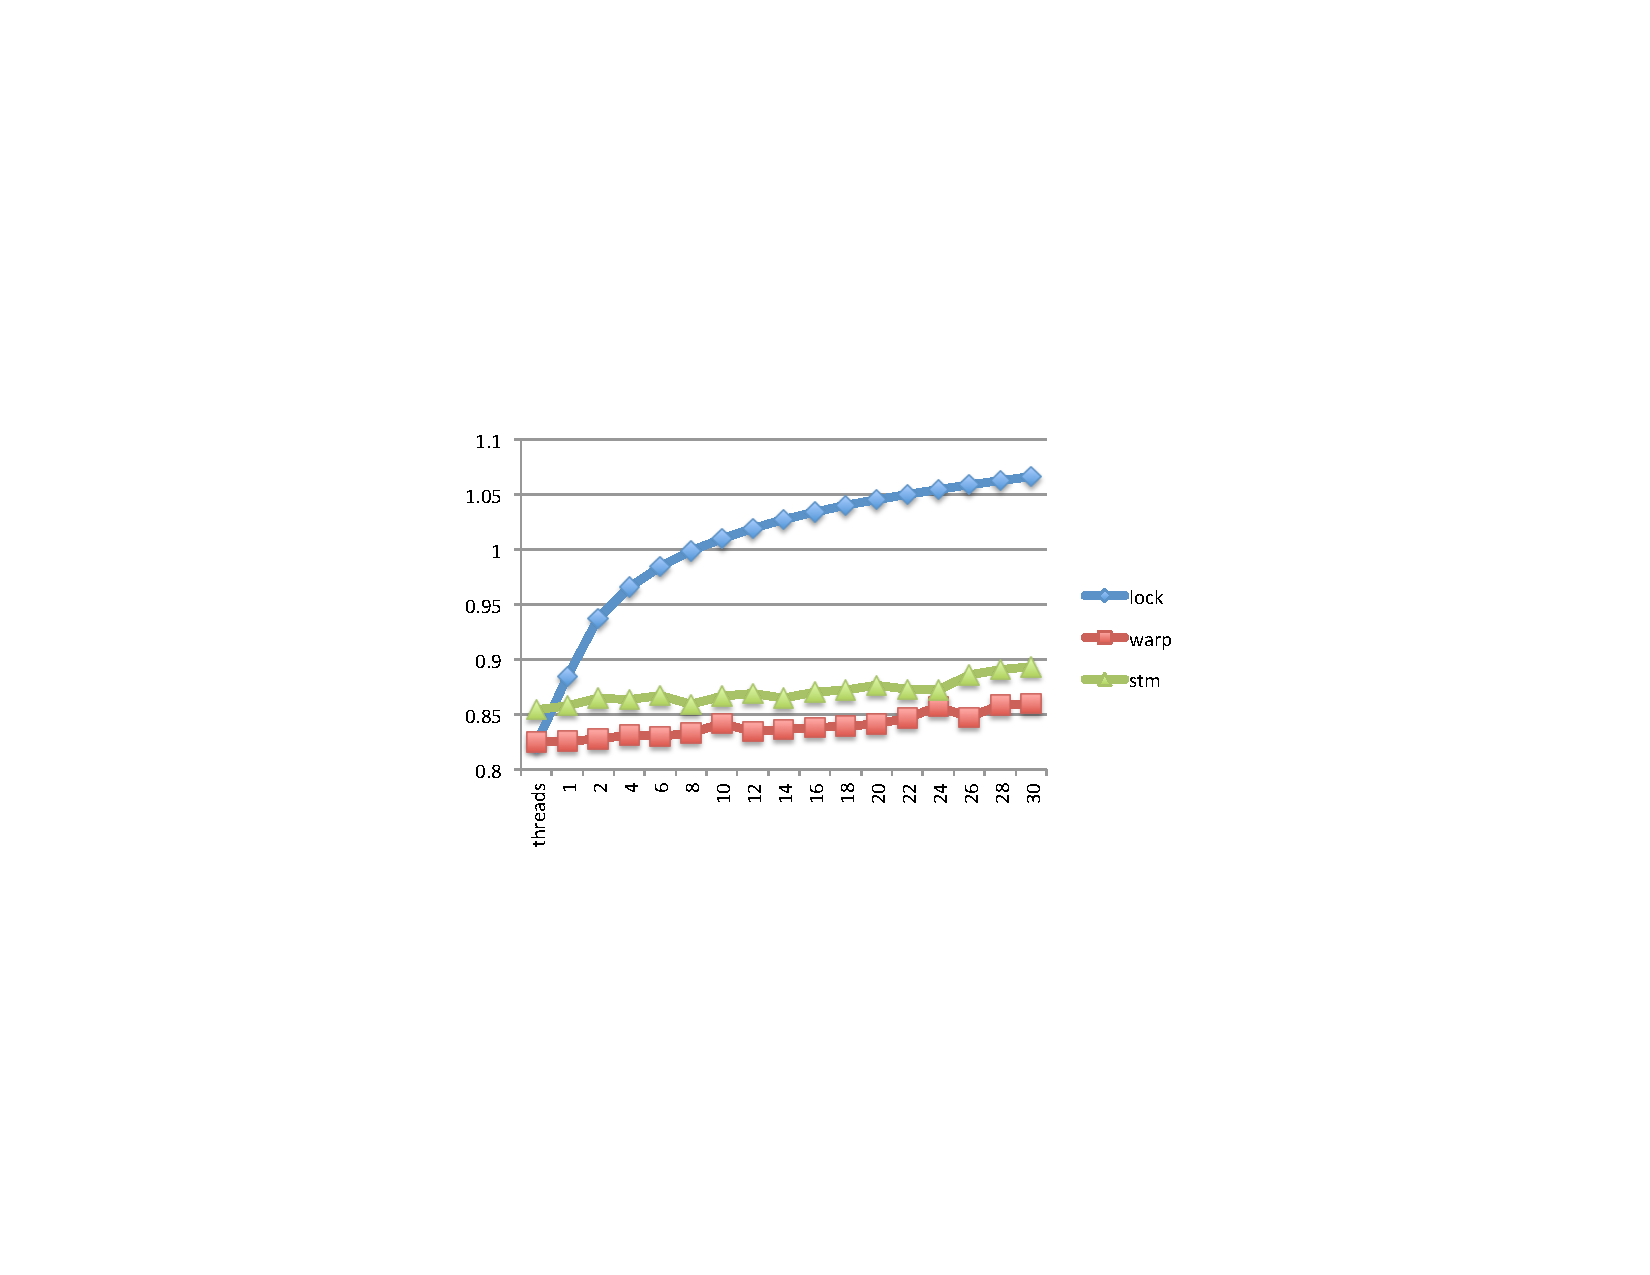
\includegraphics[width=\mywidth]{../../eval/32threads/case4th.pdf}
  \caption{\label{fig:perf} Performance results across the four subjects, measuring impact of
    workload (on the left) and concurrecny (on the right).}
\end{figure*}

  %% \vspace{-0.8cm}\caption{\label{Fi:case1th}Apache(l: workload; r: conc)\vspace{-0.2cm}}
  %% \vspace{-0.8cm}\caption{\label{Fi:case2th} 
  %%   (l: workload; r: conc)\vspace{-0.2cm}}
  %% \vspace{-0.8cm}\caption{\label{Fi:case3th}
  %%       		(l: workload; r: conc)\vspace{-0.2cm}}
  %% \vspace{-0.8cm}\caption{\label{Fi:case4th}
  %%   (l: workload; r: conc)\vspace{-0.2cm}}


\smartpar{Discussion}
%
An interesting observation w.r.t. the raw performance results is that while corrective synchronization provides stable and consistent performance improvement across all benchmarks, STM seems to do much worse on Tomcat compared to all other benchmarks. We have analyzed this gap.
%
The reason for this discrepancy,is that in both dyuproject and Flexive and Gridkit, once a first transaction manages to update the value corresponding to the input key, all other (nonoverlapping) transactions effectively become read-only transactions, and so conflict free. Hence STM achieves significant improvement compared to locks. In the case of Tomcat, however, this pattern does not hold. Transactions throughout the entire run perform write operations, leading to conflicts that degrade the performance of STM.

Interestingly, even on the benchmarks other than Tomcat STM is not able to compete with the low overhead, and thus better performance, of corrective synchronization. We suspect that the reason is that STM has to instrument memory accesses, whereas corrective synchronization applies state corrections directly.

\vfill
